\documentclass[11pt,a4paper]{article}
\usepackage[T1]{fontenc}
\usepackage[utf8]{inputenc}
\usepackage[margin=2.2cm]{geometry}
\usepackage{microtype}
\usepackage{graphicx}
\usepackage{hyperref}
\usepackage{tikz}
\usetikzlibrary{positioning,arrows.meta,fit,calc,shapes.geometric}
\usepackage{caption}
\usepackage{enumitem}
\usepackage{parskip}
\hypersetup{colorlinks=true,linkcolor=blue,urlcolor=blue,citecolor=blue}

\title{\textbf{QUIZZERA} --- Authentication Architecture\\
\large Firebase, MongoDB, and Token Flows}
\author{Engineering reference (generated for this repository)}
\date{\today}

\begin{document}
\maketitle
\tableofcontents
\vspace{1em}

\begin{abstract}
\noindent
This note describes how QUIZZERA separates \emph{identity} (Firebase Authentication)
from \emph{application profile} data stored in MongoDB (roles, account status,
onboarding, billing identifiers). It summarizes Firebase ID tokens and refresh tokens,
how the Next.js frontend interacts with them, how the API gateway routes requests,
and how the auth-service verifies callers before issuing mutations such as logout.
\end{abstract}

% -----------------------------------------------------------------------------
\section{Principles}

\begin{itemize}[leftmargin=*]
  \item \textbf{Firebase Authentication} creates accounts and issues cryptographic credentials:
        signed JWT \emph{ID tokens} and long-lived \emph{refresh tokens} used only by trusted flows.
  \item \textbf{MongoDB} stores domain-owned records keyed by \texttt{firebaseUid}.
        Firebase UID is the primary bridge between identity and profile documents.
  \item \textbf{Gateway (Express proxy)} exposes unified URLs such as
        \texttt{/api/auth/...} and forwards them to service-internal prefixes such as \texttt{/auth/...}.
  \item \textbf{Never bake application authorization purely into Firebase Custom Claims alone}
        while Mongo remains authoritative for roles/plans in this architecture --- Firebase verifies identity;
        Mongo (via sync endpoints or hydrated lookups) supplies entitlement-aware profile fields for UX/API responses.
\end{itemize}

% -----------------------------------------------------------------------------
\section{What Each Token Is}

\subsection*{Firebase ID token}
\begin{itemize}[leftmargin=*]
  \item Short-lived JWT proving ``who signed in''; verified server-side with the Firebase Admin SDK
        (\texttt{verifyIdToken}).
  \item Sent by browsers/API clients as \texttt{Authorization: Bearer \textless{}id\_token\textgreater{}} when endpoints require authentication (example in codebase: logout middleware chain).
\end{itemize}

\subsection*{Firebase refresh token}
\begin{itemize}[leftmargin=*]
  \item Opaque refresh credential returned alongside the ID token for flows that obtain tokens via REST
        (Identity Toolkit / Secure Token API).
  \item Used only with Firebase's token endpoint to obtain a fresh ID token (and optionally a rotated refresh token).
  \item The auth-service implements server-side refresh using \texttt{securetoken.googleapis.com}.
\end{itemize}

\subsection*{MongoDB user document}
\begin{itemize}[leftmargin=*]
  \item Fields include \texttt{firebaseUid}, \texttt{email}, \texttt{role}, \texttt{accountStatus}, etc.
  \item Created or linked after Firebase identity exists (register, login sync, Google token sync, guest signup).
\end{itemize}

% -----------------------------------------------------------------------------
\section{System overview (diagram)}

\begin{figure}[htbp]
  \centering
  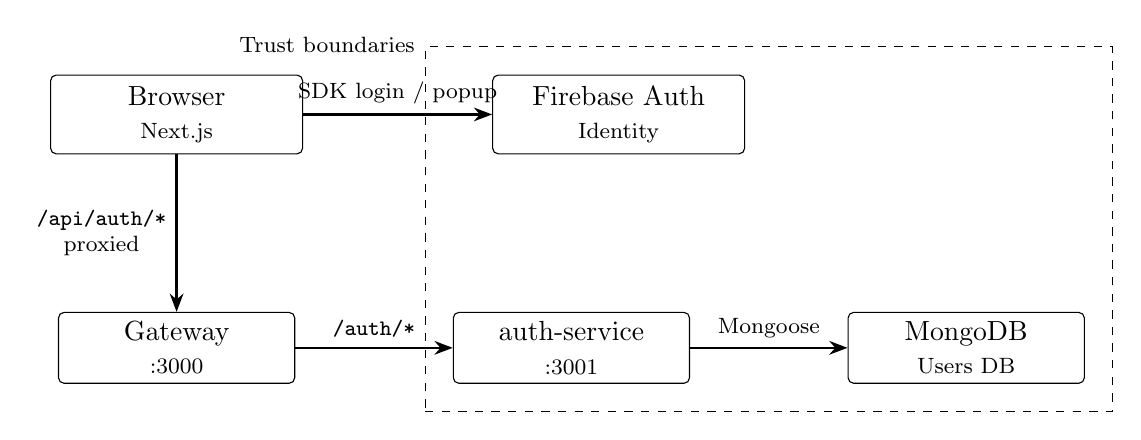
\begin{tikzpicture}[
      comp/.style={draw, rounded corners=2pt, minimum width=3.2cm, minimum height=1cm, align=center},
      svc/.style={draw, rounded corners=2pt, minimum width=3cm, minimum height=0.9cm, align=center},
      >=Stealth
    ]
    \node[comp] (browser) {Browser\\\footnotesize Next.js};
    \node[comp, right=2.4cm of browser] (firebase) {Firebase Auth\\\footnotesize Identity};
    \node[svc, below=2cm of browser] (gateway) {Gateway\\\footnotesize :3000};
    \node[svc, right=2cm of gateway] (auth) {auth-service\\\footnotesize :3001};
    \node[svc, right=2cm of auth] (mongo) {MongoDB\\\footnotesize Users DB};

    \draw[->,thick] (browser) -- node[midway,above,font=\footnotesize] {SDK login / popup}
      (firebase);
    \draw[->,thick] (browser.south) -- node[midway,left,font=\footnotesize,align=center]
      {\texttt{/api/auth/*}\\proxied}
      (gateway.north);
    \draw[->,thick] (gateway) -- node[midway,above,font=\footnotesize] {\texttt{/auth/*}}
      (auth);
    \draw[->,thick] (auth) -- node[midway,above,font=\footnotesize] {Mongoose}
      (mongo);

    \node[draw,dashed,inner sep=10pt,fit=(firebase)(auth)(mongo),label={[anchor=south east,yshift=-2mm]north west:\footnotesize Trust boundaries}]
      {};
  \end{tikzpicture}
  \caption{Logical placement of components for QUIZZERA authentication.}
\end{figure}

% -----------------------------------------------------------------------------
\section{Frontend session flow (Firebase SDK path)}

The Next.js app configures Firebase Auth client SDK (email/password, Google popup, password reset email).
After Firebase establishes a session, \texttt{onAuthStateChanged} obtains an ID token via \texttt{getIdToken()}
and POSTs it through the gateway to \texttt{/api/auth/google} with JSON body \texttt{\{ idToken \}}.

\textbf{Naming note:} despite the path segment ``google'', the implementation verifies \emph{any} Firebase ID token
from the configured project (email/password users included) and performs MongoDB find-or-create by \texttt{firebaseUid}.

\begin{figure}[htbp]
  \centering
  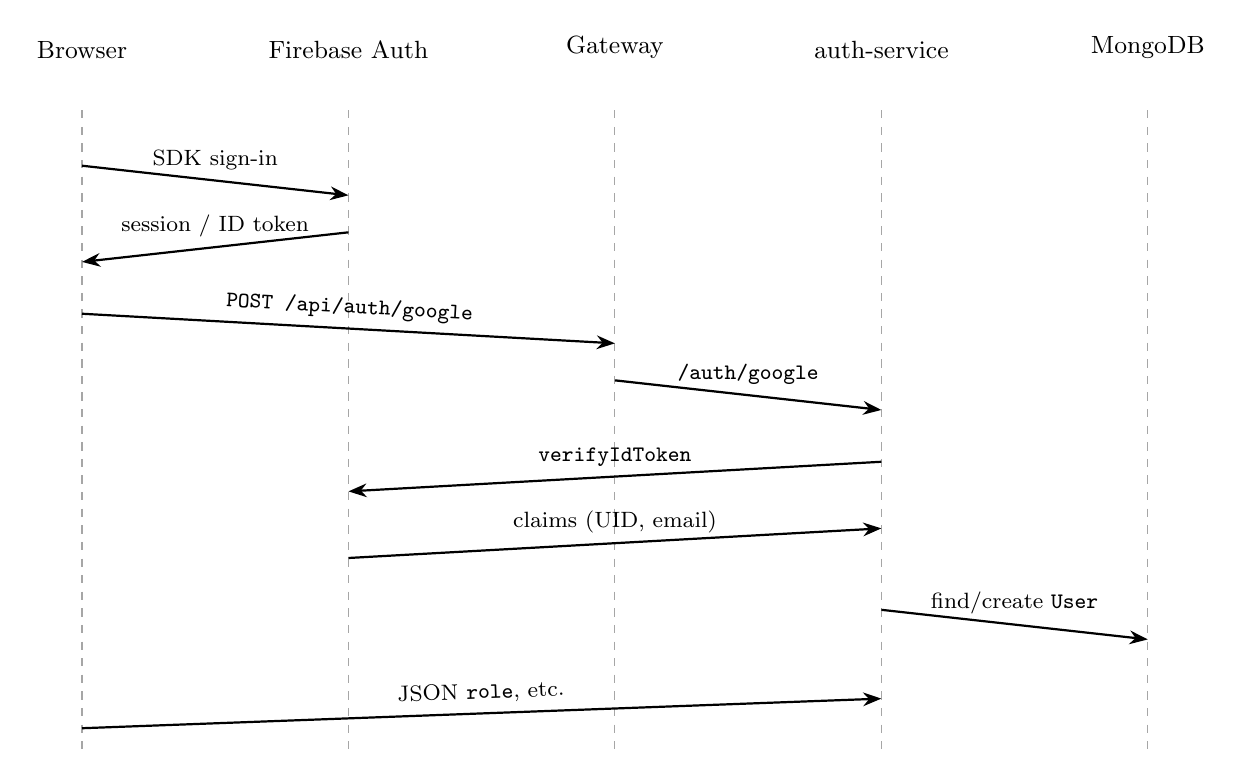
\begin{tikzpicture}[scale=0.94, every node/.style={font=\small}, >=Stealth]
    % Lifeline x-positions (cm)
    \coordinate (L0) at (0,0);
    \coordinate (L1) at (3.6,0);
    \coordinate (L2) at (7.2,0);
    \coordinate (L3) at (10.8,0);
    \coordinate (L4) at (14.4,0);

    \node[above=2mm] at (L0) {Browser};
    \node[above=2mm] at (L1) {Firebase Auth};
    \node[above=2mm] at (L2) {Gateway};
    \node[above=2mm] at (L3) {auth-service};
    \node[above=2mm] at (L4) {MongoDB};

    \foreach \n in {L0,L1,L2,L3,L4}
      \draw[dashed,gray!70] ($(\n)+(0,-0.35)$) -- ($(\n)+(0,-9)$);

    % Messages (down the page)
    \draw[->,thick] ($(L0)+(0,-1.1)$) -- node[above,font=\footnotesize] {SDK sign-in}
      ($(L1)+(0,-1.5)$);
    \draw[->,thick] ($(L1)+(0,-2.0)$) -- node[above,font=\footnotesize] {session / ID token}
      ($(L0)+(0,-2.4)$);

    \draw[->,thick] ($(L0)+(0,-3.1)$) -- node[above,font=\footnotesize,sloped]
      {\texttt{POST /api/auth/google}} ($(L2)+(0,-3.5)$);
    \draw[->,thick] ($(L2)+(0,-4.0)$) -- node[above,font=\footnotesize]
      {\texttt{/auth/google}} ($(L3)+(0,-4.4)$);

    \draw[->,thick] ($(L3)+(0,-5.1)$) -- node[above,font=\footnotesize]
      {\texttt{verifyIdToken}} ($(L1)+(0,-5.5)$);
    \draw[<-,thick] ($(L3)+(0,-6.0)$) -- node[above,font=\footnotesize]
      {claims (UID, email)} ($(L1)+(0,-6.4)$);

    \draw[->,thick] ($(L3)+(0,-7.1)$) -- node[above,font=\footnotesize]
      {find/create \texttt{User}} ($(L4)+(0,-7.5)$);

    \draw[<-,thick] ($(L3)+(0,-8.3)$) -- node[above,font=\footnotesize,sloped]
      {JSON \texttt{role}, etc.} ($(L0)+(0,-8.7)$);
  \end{tikzpicture}
  \caption{Simplified sequence for browser-driven Firebase login followed by Mongo profile sync.}
\end{figure}

% -----------------------------------------------------------------------------
\section{REST-first flows (Identity Toolkit / Secure Token)}

These endpoints live under \texttt{/auth} on the auth-service (gateway path \texttt{/api/auth/...}).

\subsection*{Register (\texttt{POST /auth/register})}
Firebase Admin creates the Firebase user with email/password; Mongo creates \texttt{User} with matching \texttt{firebaseUid}.
Rollback deletes Firebase user if Mongo creation fails.

\subsection*{Login (\texttt{POST /auth/login})}
Server calls Identity Toolkit \texttt{accounts:signInWithPassword}, receives \texttt{idToken} + \texttt{refreshToken},
links/creates Mongo user by \texttt{localId}.

\subsection*{Refresh (\texttt{POST /auth/refresh})}
Body carries refresh token; server exchanges it at Secure Token API for a new ID token (and optional rotated refresh).

\subsection*{Logout (\texttt{POST /auth/logout})}
Requires \texttt{Bearer} ID token; middleware verifies JWT then loads Mongo user; service revokes Firebase refresh tokens for that UID.

\begin{figure}[htbp]
  \centering
  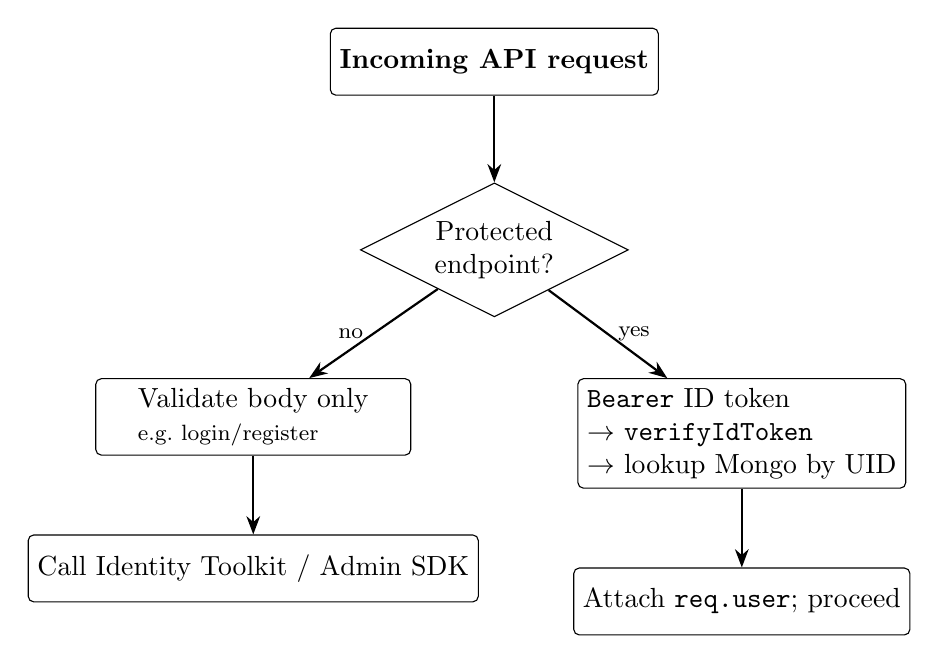
\begin{tikzpicture}[
      rect/.style={draw, rectangle, rounded corners=2pt, minimum height=0.85cm, minimum width=4cm, align=left},
      decide/.style={draw, diamond, aspect=2, inner sep=2pt, align=center},
      >=Stealth
    ]
    \node[rect] (req) {\textbf{Incoming API request}};
    \node[decide,below=1.1cm of req] (prot) {Protected\\endpoint?};
    \node[rect,below left=1.2cm and 0.2cm of prot] (nop) {Validate body only\\\footnotesize e.g.\ login/register};
    \node[rect,below right=1.2cm and 0.2cm of prot] (yes) {\texttt{Bearer} ID token\\
      $\rightarrow$ \texttt{verifyIdToken}\\
      $\rightarrow$ lookup Mongo by UID};
    \node[rect,below=1cm of nop] (svc) {Call Identity Toolkit / Admin SDK};
    \node[rect,below=1cm of yes] (hdl) {Attach \texttt{req.user}; proceed};

    \draw[->,thick] (req) -- (prot);
    \draw[->,thick] (prot) -- node[left,font=\footnotesize] {no} (nop);
    \draw[->,thick] (prot) -- node[right,font=\footnotesize] {yes} (yes);
    \draw[->,thick] (nop) -- (svc);
    \draw[->,thick] (yes) -- (hdl);
  \end{tikzpicture}
  \caption{High-level decision at the boundary of auth-service routes.}
\end{figure}

% -----------------------------------------------------------------------------
\section{Operational checklist}

\begin{enumerate}[leftmargin=*]
  \item Ensure Firebase Web API key and Admin credentials are configured where server routes call Identity Toolkit / Secure Token / Admin verify.
  \item Ensure Mongo connection string is reachable (Atlas IP allowlist / VPC rules).
  \item Ensure gateway env URLs match running service ports (\texttt{AUTH\_SERVICE\_URL} defaults to localhost:3001).
  \item Password reset emails use Firebase client \texttt{sendPasswordResetEmail}; template and authorized domains must be valid in Firebase Console.
\end{enumerate}

\vfill
\noindent\textit{Build this PDF with} \texttt{pdflatex quizzera-auth-architecture.tex} \textit{(run twice for stable references).}

\end{document}
